\documentclass[12pt]{article}
\usepackage{geometry}                % See geometry.pdf to learn the layout options. There are lots.
\geometry{letterpaper}                   % ... or a4paper or a5paper or ... 
%\geometry{landscape}                % Activate for for rotated page geometry
\usepackage[parfill]{parskip}    % Activate to begin paragraphs with an empty line rather than an indent
\usepackage{daves,fancyhdr,natbib,graphicx,dcolumn,amsmath,lastpage,url}
\usepackage{amsmath,amssymb,epstopdf,longtable}
\usepackage{paralist} 
\DeclareGraphicsRule{.tif}{png}{.png}{`convert #1 `dirname #1`/`basename #1 .tif`.png}
\pagestyle{fancy}
\lhead{CE 3372 -- Water Systems Design}
%\rhead{FALL 2010}
%\rhead{SPRING 2011}
%\rhead{FALL 2011}
%\rhead{SPRING 2012}
%\rhead{FALL 2013}
%\rhead{FALL 2016}
\rhead{FALL 2017}
%\lfoot{EXERCISE 1 -- REVISION 1}
%\lfoot{EXERCISE 1 -- REVISION 2}
%\lfoot{EXERCISE 1 -- REVISION 3}
\lfoot{ES 21}
\cfoot{}
\rfoot{Page \thepage\ of \pageref{LastPage}}
\renewcommand\headrulewidth{0pt}



\begin{document}

\begin{center}
\textbf{MEMORANDUM}
%{\textbf{{ CE 3372 -- Water Systems Design} \\ {Exercise Set 2}}}
\end{center}
\begingroup
\begin{tabular}{p{1in} p{5in}}
\hline
\hline
To: & P. N Guin \\ ~\\
From: & P. Olar Bear \\ ~\\
Date: & 04MAR2024 \\ ~\\
Subject: & CE 3372 -- Water Systems Design, Exercise Set 21. ~\\

\hline
\hline
\end{tabular}
\endgroup


\section*{\small{Purpose}}
The purpose of the exercise(the problem statement is repeated below) is to develop expertise in application of gradually varied flow equation in open channel flow, and practice SWMM skills for simple geometries.  The exercise is a repeat of an earlier exercise using SWMM instead of hand-built tools.

\section*{\small{Discussion}}
The solution is presented below after re-statement of the problem.  Relevant discussion components appear imbedded within the solution.
%%~ & ~ \\
%%ABET General Criteria 3: & (a) \dots apply knowledge of mathematics, science, and engineering  \\
%%~ & (e)  \dots solve engineering problems  \\
%%~ & (k) \dots an ability to use the techniques, skills, and modern engineering tools necessary for engineering practice. \\
%%%~ & ~ \\
%%%Grading Criteria:  & Completion; Correct Solutions; Calculation Details \\
%\end{tabular}
%\endgroup
\section*{\small{Problem Statement}}
\begin{enumerate}
%%%%%%%%%%%%%%%%%%
\item Water flows at a steady rate of 192$ft^3/s$ through a concrete-lined rectangular channel 16 ft wide as depicted in Figure \ref{fig:channel_profile}. The water enters the $0.35 \%$ sloped channel ($S_0 = 0.0035$) at location $1$ and is flowing at $110\%$ normal depth ($1.1 \times y_n$).  The water exits over a 3-foot tall weir (assume sharp-crest weir) at location $2$.

\begin{figure}[htbp] %  figure placement: here, top, bottom, or page
   \centering
   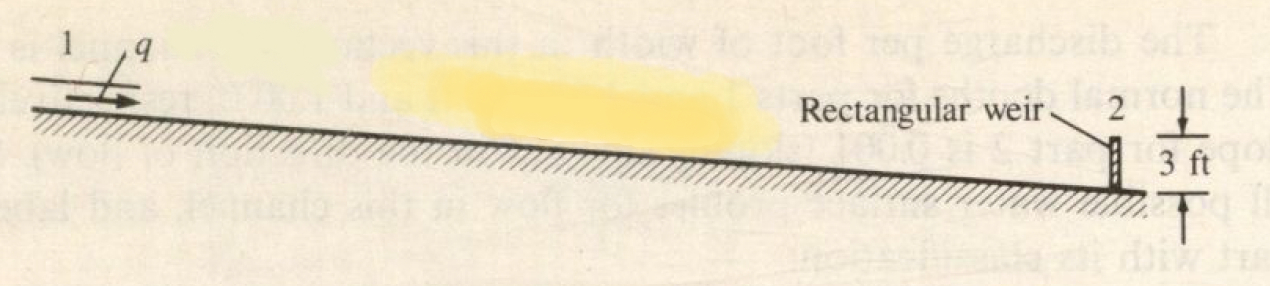
\includegraphics[width=6in]{channel_profile.jpg} 
   \caption{Profile of concrete-lined rectangular channel.}
   \label{fig:channel_profile}
\end{figure}

Use SWMM to repeat the exercise in ES-19.  The problem set-up is repeated above.  Use the average $\Delta x$ from your ES-19 solution as the spatial step in SWMM to use.

\begin{enumerate}[a)]
\item Make your SWMM model have conduits that are the average $\Delta x$ from ES-19.
\item Set the \texttt{FIXED} outfall boundary condition as the pool elevation you determined in ES-19.
\item Run the SWMM model using \texttt{DYNAMIC WAVE} routing.
\item Include a screen capture of your SWMM model showing the computed water-surface-profile.   
\item Export the water surface profile from SWMM and demonstrate that the computed profile in SWMM and in ES-19 (by-hand) are essentially the same.
\end{enumerate}



\section*{\small{Solution}}
To address the specific questions in ES-19 the following steps were required:
\begin{enumerate}
\item Build a tool to take Q, n, Width as input. Figure \ref{fig:GVF-UpperLeft} is such a tool with these inputs along the left side of the spreadsheet.
\item Compute normal and critical depth for the channel.
Normal depth is computed using Manning's equation for a rectangular channel, then apply goal seek until the computed flow rate agrees with the prescribed flow rate.  For the supplied problem values the normal depth is about 1.509 feet.  Critical depth is computed settinf the Froude number for the rectangular channel to unity (one) and solving for the required flow depth.  For the supplied problem values the critical depth is about 1.648 feet.
\item Assume depth at weir is weir height+critical depth -- use that as starting value for the numerical method.  For the supplied problem values, the pool depth just upstream of the weir is about 4.648 feet.
\item Use variable step method as outlined in class an compute spacing as depth is changed.  For the supplied values, we start at the weir and compute upstream, using depth increments of 0.1 feet until the depth is at 110\% of normal depth, which for this problem is about 1.66 feet.
%\item If there is a sign change, then there is a hydraulic jump.  Continue after the jump, but remember to reverse the spacings for the plots.
\item Plot the results.
\end{enumerate}

Implementing these steps was shown in Figure \ref{fig:GVF-UpperLeft}.

\begin{figure}[htbp] %  figure placement: here, top, bottom, or page
   \centering
   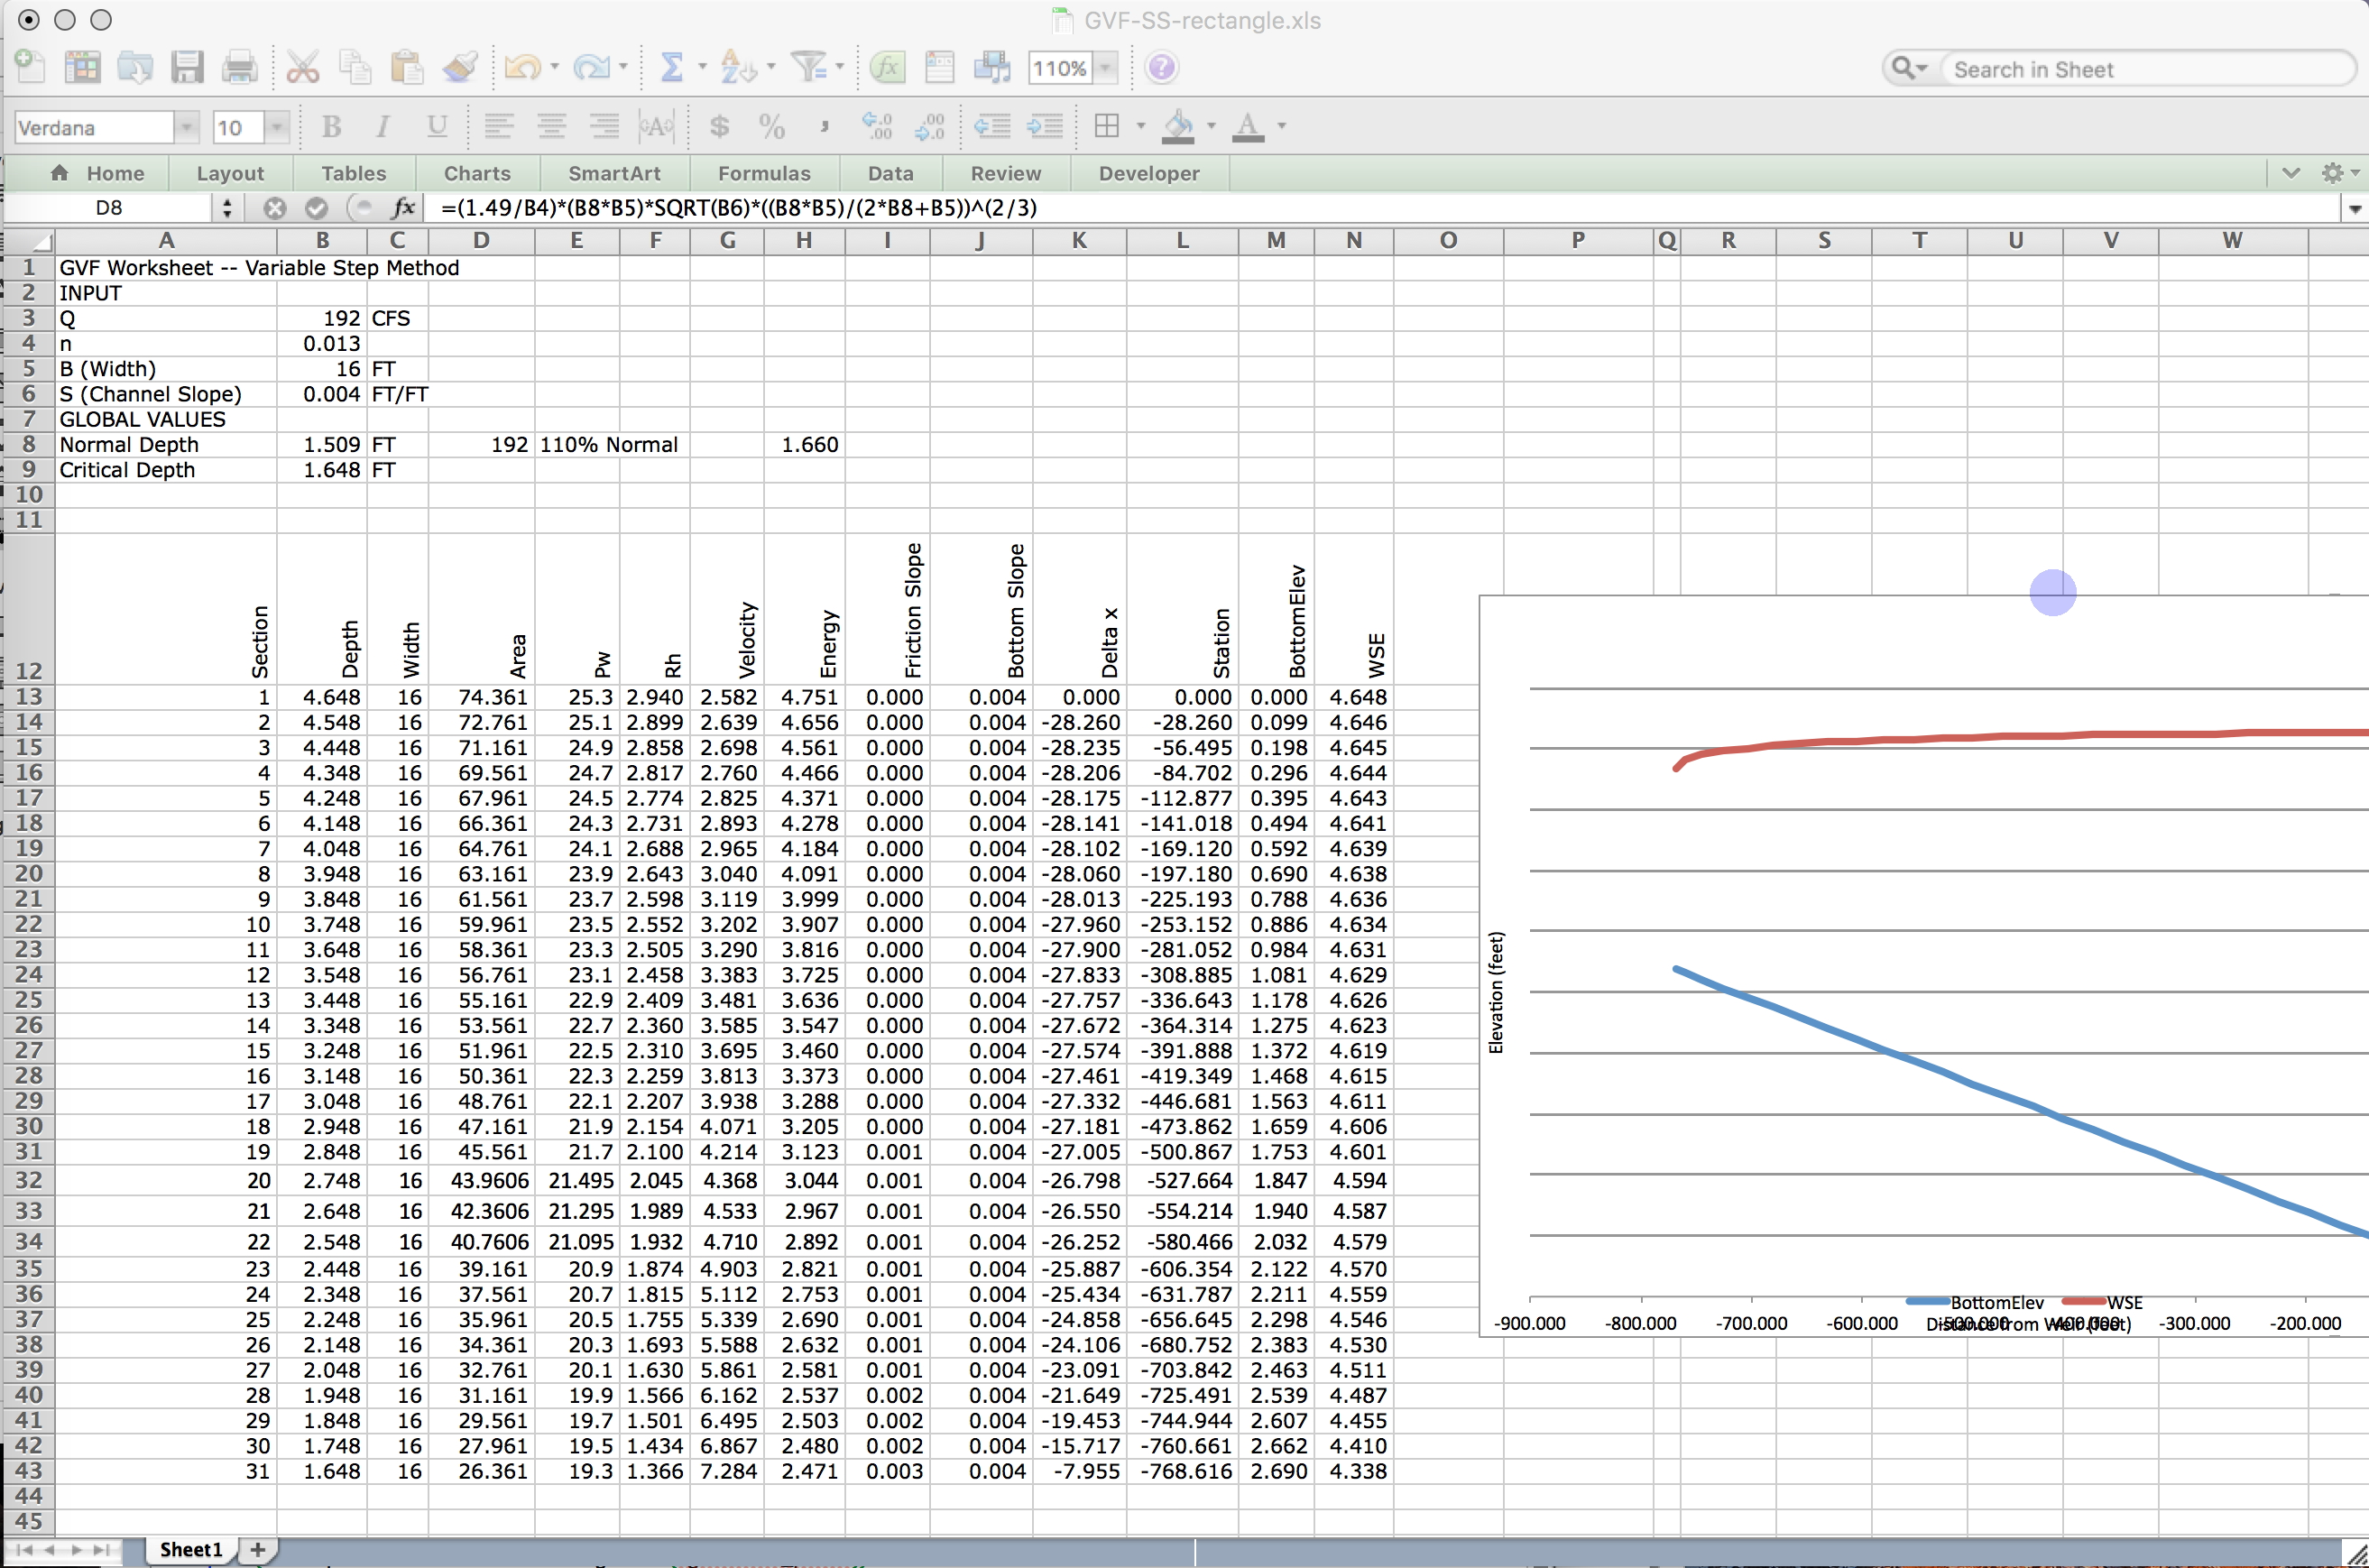
\includegraphics[width=4in]{GVF-UpperLeft.jpg} 
   \caption{GVF Spreadsheet for channel in Figure\ref{fig:channel_profile}}
   \label{fig:GVF-UpperLeft}
\end{figure}

The average spacing can be estimated as the total distance $\approx 768 ft.$ divided by the number of reaches (in this solution 30), which is $\approx 25.6 ft.$.   Use this value in the next exercise where the same problem is examined using SWMM. 


\begin{figure}[htbp] %  figure placement: here, top, bottom, or page
   \centering
   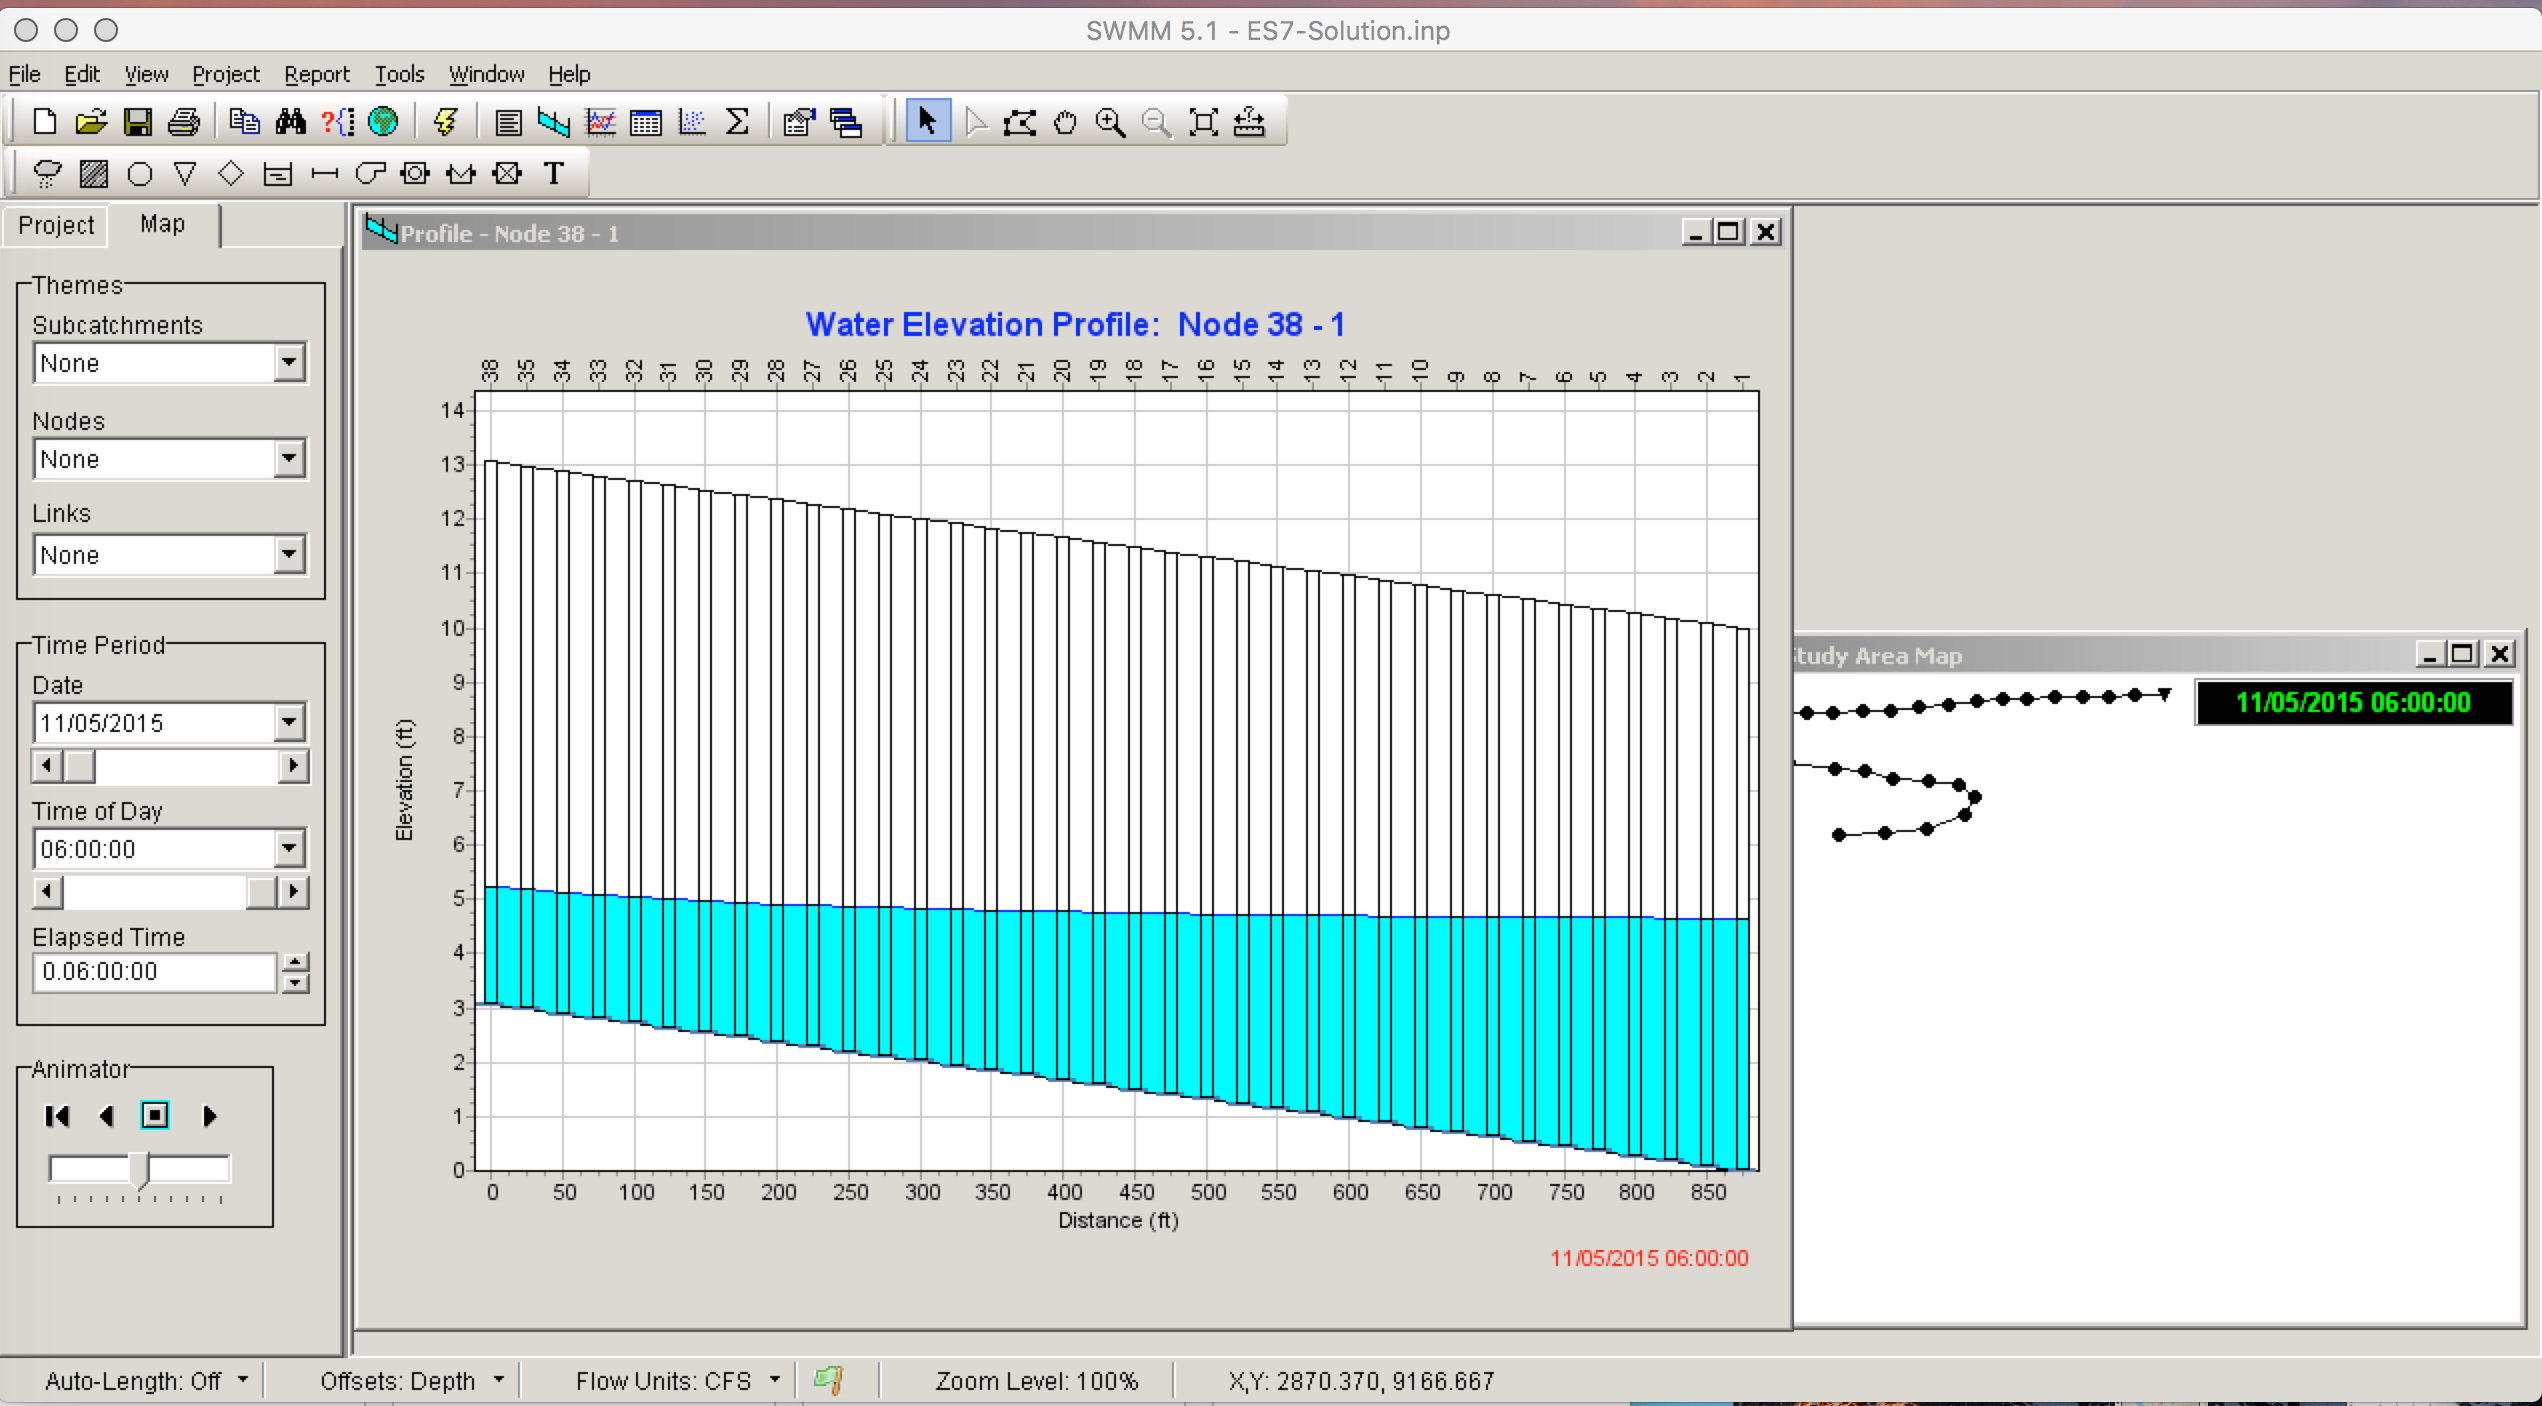
\includegraphics[width=4in]{SWMM-WSP.jpg} 
   \caption{GVF Spreadsheet for channel in Figure\ref{fig:channel_profile}}
   \label{fig:SWMM-WSP}
\end{figure}

Figure \ref{fig:SWMM-WSP} is a screen capture of a SWMM model to replicate the problem conditions. 
At first glance the profiles look identical (they are not, but they are close).

\begin{figure}[htbp] %  figure placement: here, top, bottom, or page
   \centering
   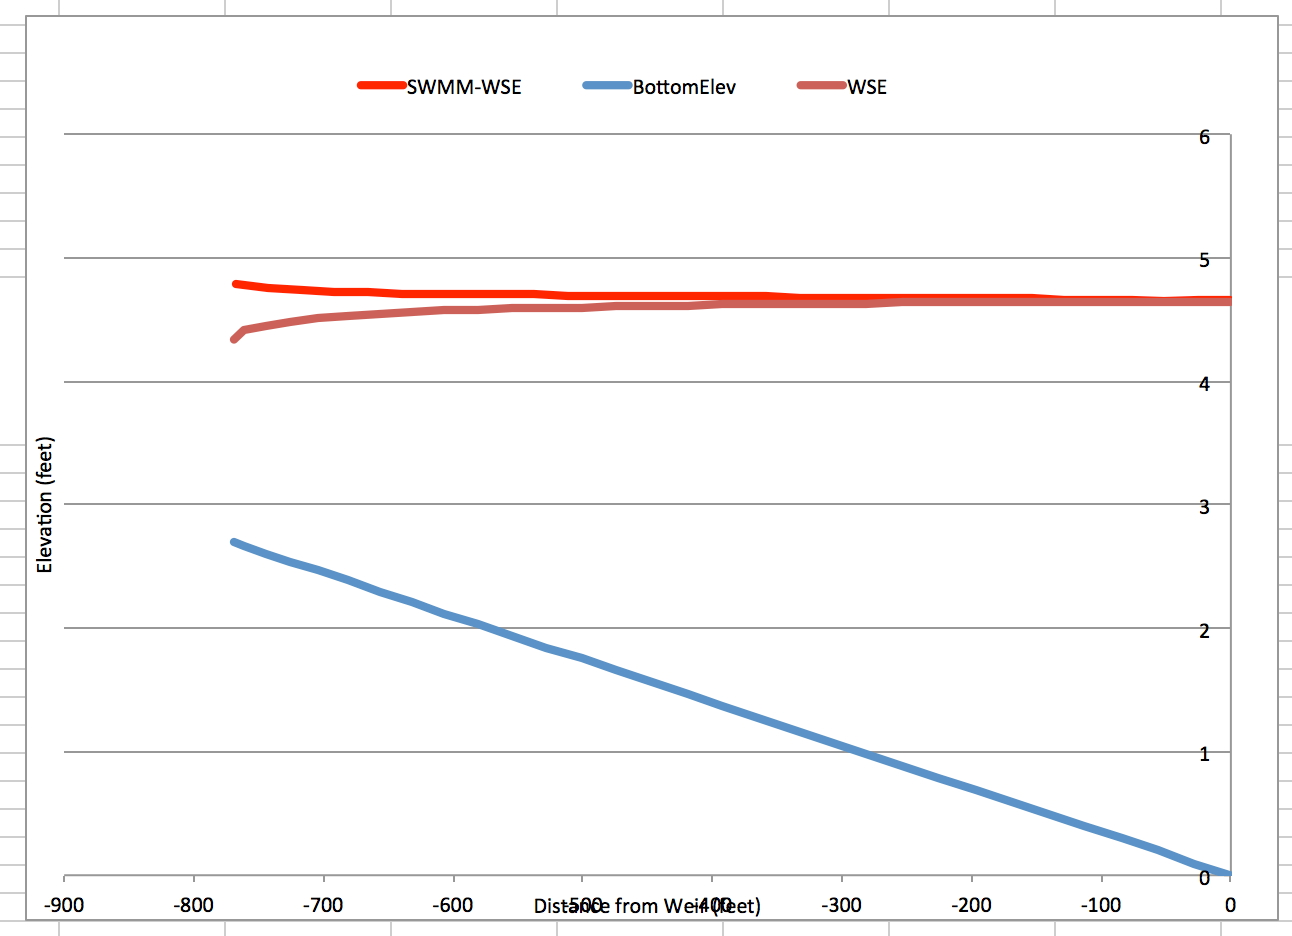
\includegraphics[width=5in]{SWMM-WSP2.jpg} 
   \caption{Comparison of SWMM and by-hand solutions}
   \label{fig:SWMM-WSP2}
\end{figure}

Figure \ref{fig:SWMM-WSP2} is a plot that displays both profiles on the same axes.  
The profiles are similar close to the downstream pool, but depart at the upstream end --- but not by much; either would be meaningful for engineering decisions.  
The result indicates that the gradually varied flow equation is conceptually simple (as evidenced by the step-backwater method in Excel), but in practice one would choose to use the professional program (as much for acceptance of results as other inherent error checking that is completely omitted from our by-hand technique).
\end{enumerate}
\end{document}  